\subsubsection{ Digit readers }

\begin{itemize}

\item For each $i = 1,2,3$,
               $j = 0,\ldots,l-3$,
               $u \in \{0, 1\}^j$, and
               $\inc \in \{{\tt increment}, {\tt copy} \}$:
    \begin{itemize}
        \item if $j = 0$:
        create
        $\begin{aligned}[t]
            \dreader(& \left\langle {\tt Read}, i, \lambda, \inc \right\rangle,
                       \left\langle {\tt Read}, i, 0, \inc \right\rangle,
                       \left\langle {\tt Read}, i, 1, \inc \right\rangle \;)
        \end{aligned}$\\ from the general gadget in Figure~\ref{fig:digit_read}.

        \item else:
        create
        $\begin{aligned}[t]
        \dreader(& \left\langle {\tt Read}, i, u,  \inc \right\rangle,
                   \left\langle {\tt Read}, i, 0u, \inc \right\rangle,
                   \left\langle {\tt Read}, i, 1u, \inc \right\rangle \;)
        \end{aligned}$\\ from the general gadget in Figure~\ref{fig:digit_read}.
    \end{itemize}

\end{itemize}

For each $i = 1,2,3$ and each $u \in \{0, 1\}^{l-2}$
\begin{itemize}

    \item Create
        $\begin{aligned}[t]
            \dreader(& \left\langle {\tt Read},    i,  u, {\tt copy} \right\rangle,
                       \left\langle {\tt PreWarp}, i, 0u, {\tt copy} \right\rangle,
                       \left\langle {\tt PreWarp}, i, 1u, {\tt copy} \right\rangle \;)
        \end{aligned}$\\from the general gadget in Figure~\ref{fig:digit_read}.

    \item Let $guess0$ = 0$u$, $guess1$ = 1$u$

    if $4 \cdot (dec(guess0) + 1) < m - 1$

    then $R0$ = $bin(4 \cdot dec(guess0) + 1)+u[1]+u[0], {\tt copy}$

    else $R0$ = $\{0 \}^l, {\tt increment}$

    \vspace{.5cm}

    if $4 \cdot (dec(guess1) + 1) < m - 1$

    then $R1$ = $bin(4 \cdot dec(guess1) + 1)+u[1]+u[0], {\tt copy}$

    else $R1$ = $\{0 \}^l, {\tt increment}$

    \vspace{.5cm}

    Create
    $\begin{aligned}[t]
        \dreader(& \left\langle {\tt Read},    i,  u, {\tt increment} \right\rangle,
                   \left\langle {\tt PreWarp}, i, R0 \right\rangle,
                   \left\langle {\tt PreWarp}, i, R1 \right\rangle \;)
    \end{aligned}$\\from the general gadget in Figure~\ref{fig:digit_read}.

\end{itemize}

\begin{figure}[H]
    \centering
    \begin{subfigure}[t]{0.2\textwidth}
        \centering
        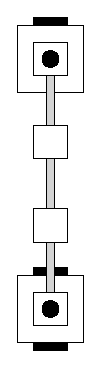
\includegraphics[width=0.2\textwidth]{read/read_0}
        \caption{\label{fig:read_0} {\tt Read\_0}}
    \end{subfigure}%
    ~
    \begin{subfigure}[t]{0.2\textwidth}
        \centering
        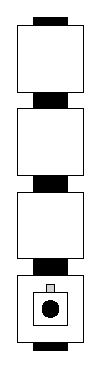
\includegraphics[width=0.2\textwidth]{read/read_1}
        \caption{\label{fig:read_1} {\tt Read\_1}}
    \end{subfigure}%
    \caption{\label{fig:digit_read} {\tt Read} gadgets}
\end{figure}
